\subsection{Pipeline Join on Compressed Data}\label{sec:match_join}
\begin{figure}[ht]
  \centering
  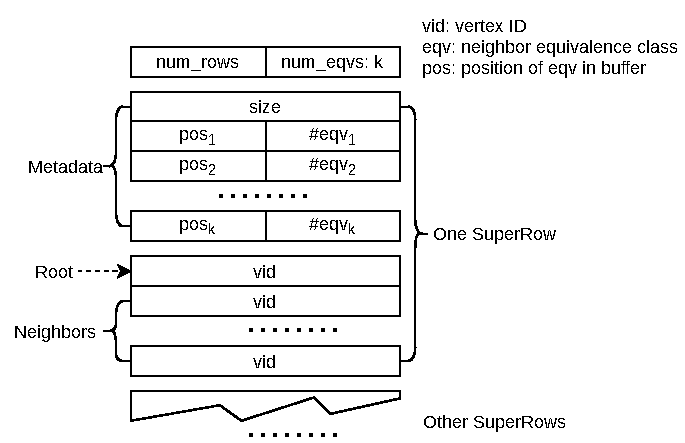
\includegraphics[width=0.32\textwidth]{img/compress.pdf}
  \caption{The disk format of our compressed star matching results.}\label{img:compress}
\end{figure}

By far, we've got all the compressed matching results for stars and it's time to join them to obtain the final answer.
A simple and straightforward method is the binary join, however, intermediate join results have to be materialized by doing so.
Even though the compression ratio of star matching result is very impressive,
the joined result could expand significantly because the permutation among roots is unavoidable~\cite{DBLP:journals/pvldb/SunWWSL12}.
To address this problem, we propose a indexed pipeline join algorithm on compressed data:

Consider the SuperRow that we discussed before, whose columns are image set for \textsc{NeighborInfo} equivalence class except the first column, which is the matching result of the root.
Thus the first column of a SuperRow contains only a single vertex, which is suitable for the key of a index.
In fact, the index is generated during the star matching process,
for each SuperRow we append the root id and the position of it to the index file.
With this index, we are able to locate to the corresponding SuperRows efficiently during the join process.

The basic structure of our pipeline join is a series of nested loops.
However, unlike the traditional join problem, we join on image sets rather than single elements,
which means set intersection is the most computation intensive operation.
Consider the social media network, a trending media could easily attract millions or even billions of viewers,
to join on such trending media rooted stars, we must calculate the set intersection of such enormous viewers.
A conventional hash join method could easily eat up the memory of a PC and have poor locality.
To address this problem, we provide an out-of-core sequential approach by merging on the image sets.
Therefore the image sets should be sorted otherwise the sorting operation could be another bottleneck.
In fact, with the elegant design of our vertex-centric property graph storage method,
the vertices are already sorted in the data graph, and we can implement our sequential out-of-core set intersection for free.
